\documentclass[multi=page, border=0.5cm]{standalone}
\usepackage{calculator}
\usepackage[svgnames]{xcolor}
\usepackage{tikz}

\tikzset{    
    poly/.style={ line width=2mm, red }
}

\definecolor{light-gray}{gray}{0.95}

\begin{document}
\begin{page}
    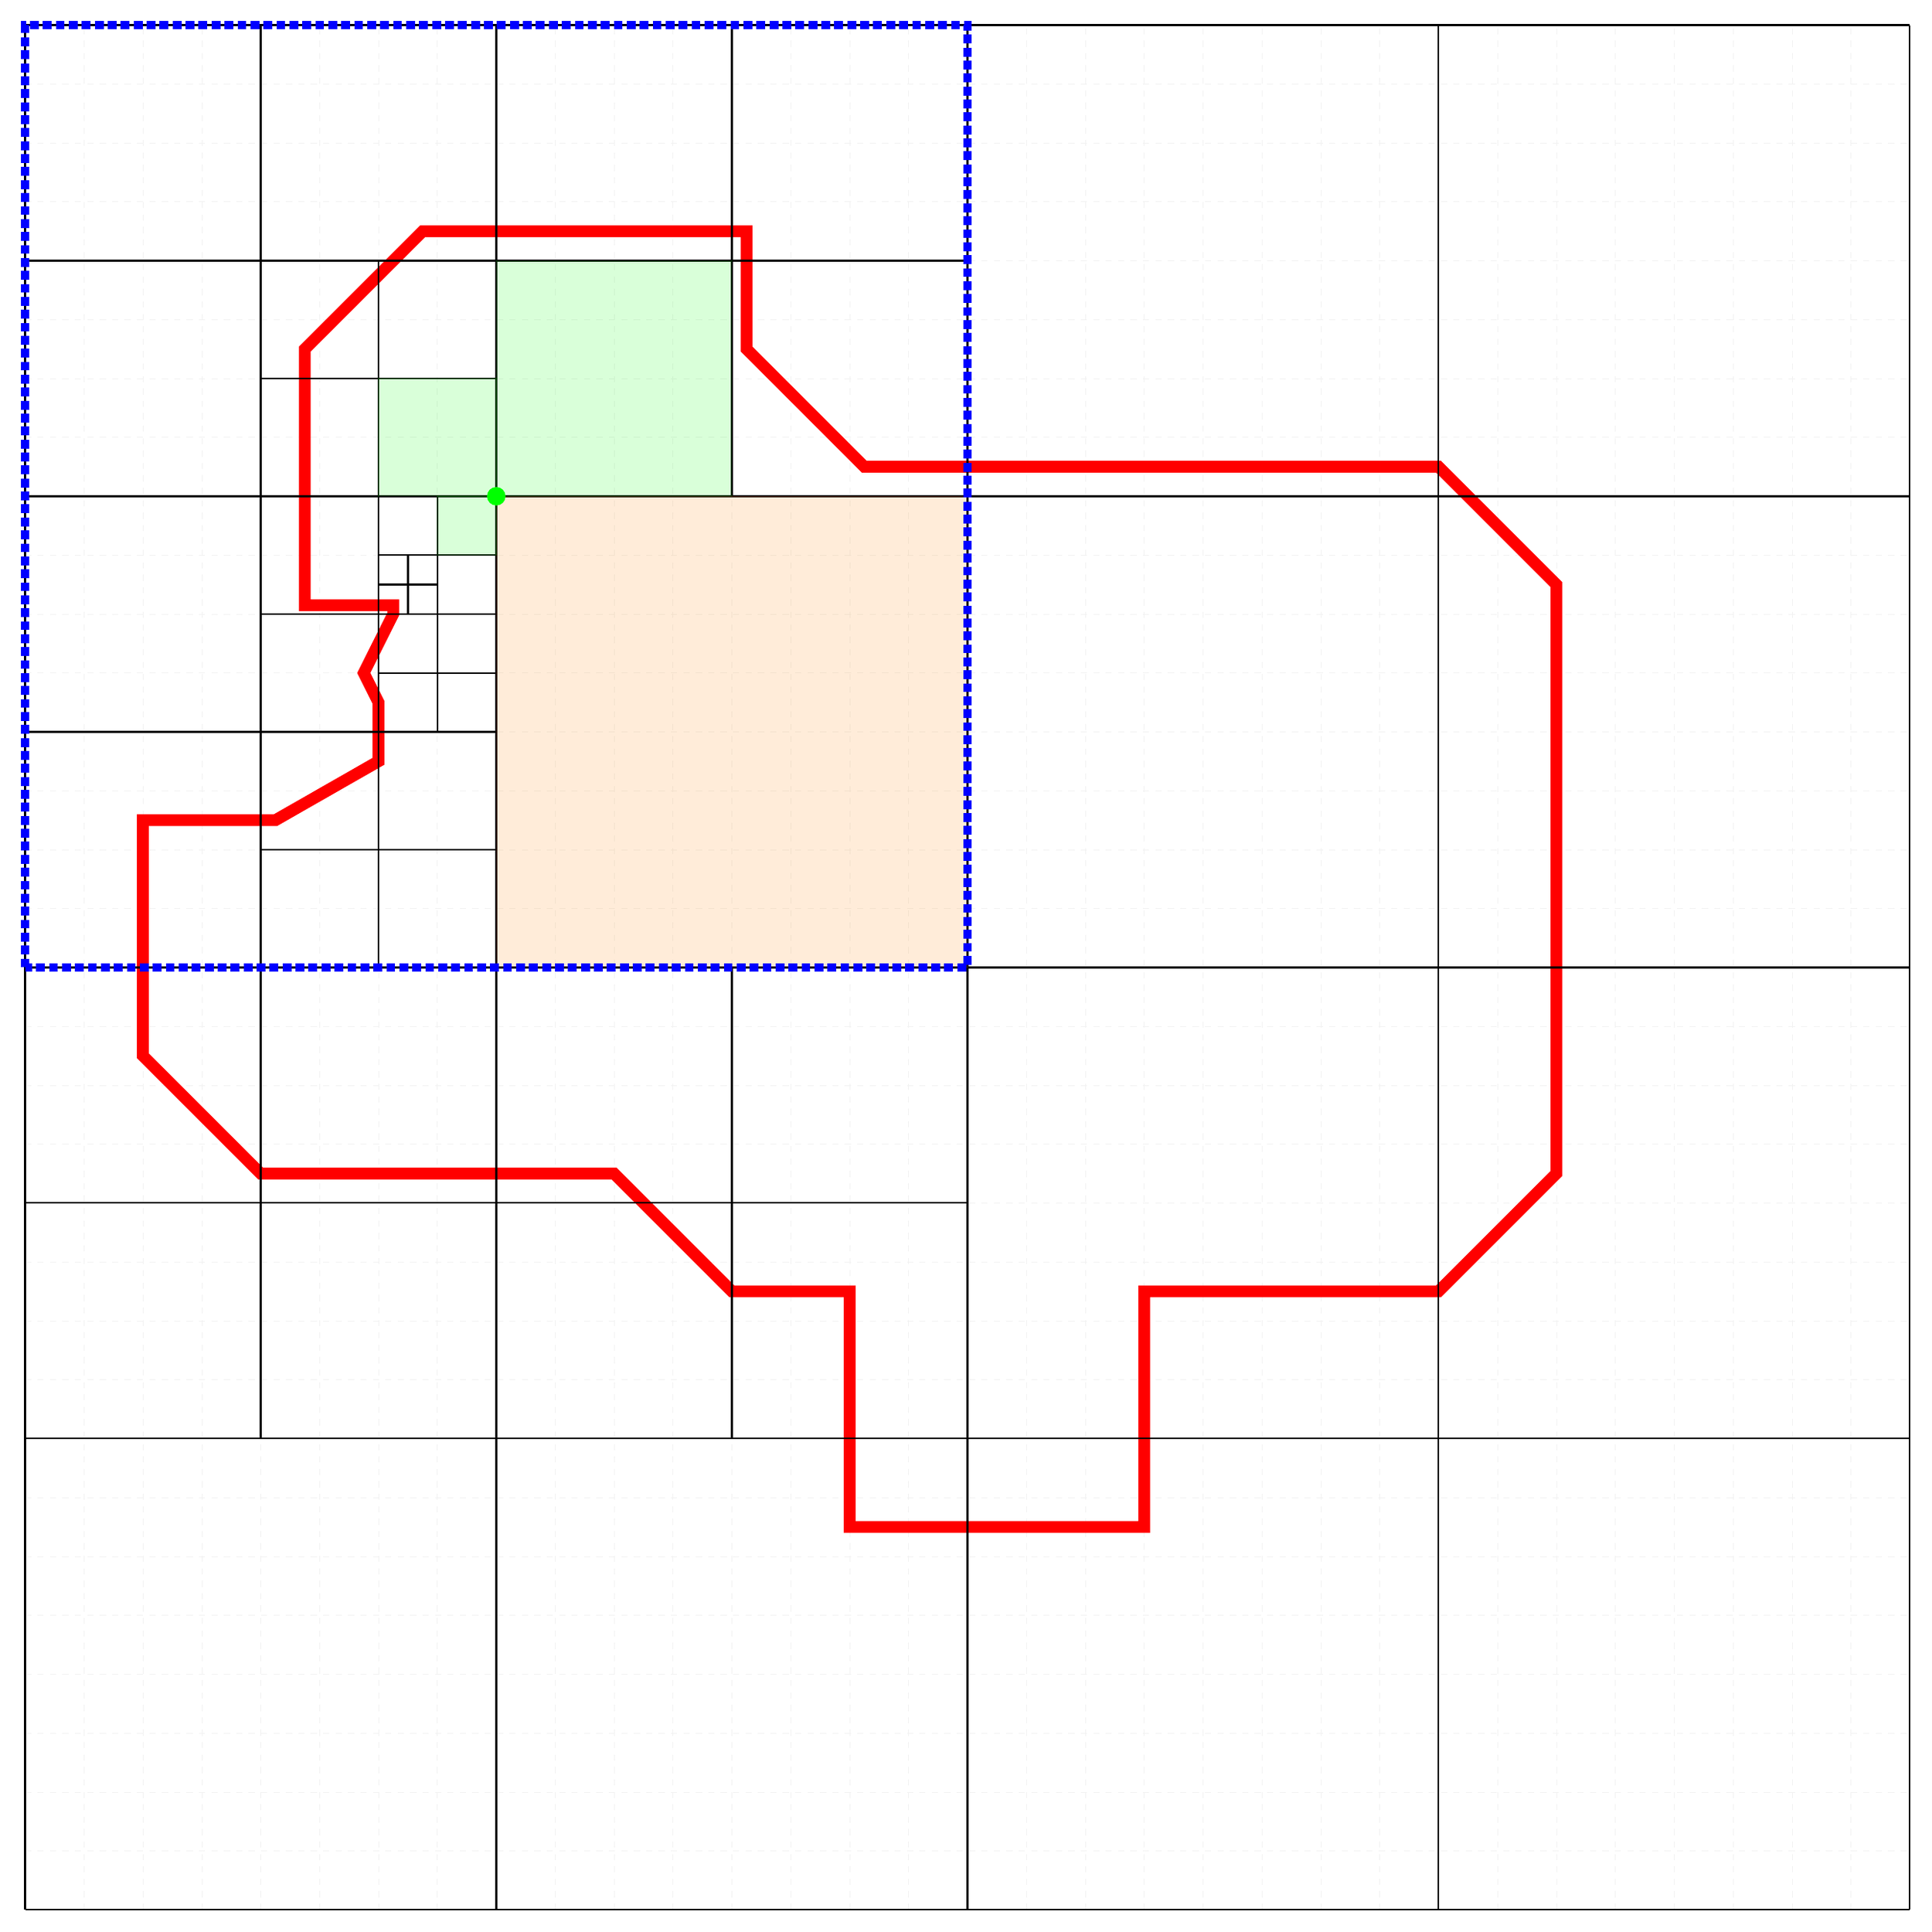
\begin{tikzpicture}
        \draw[step=1, very thin, light-gray, dashed] (0,0) grid (32,32);
        
        \node (start) at (6.25,22.25) {};
        \draw[poly] (start) -- ++(0,-0.25) -- ++(-0.25,-0.5) -- ++(-0.25,-0.5)  -- ++(0.25,-0.5)
            -- ++(0,-1) -- ++(-1.75,-1) -- ++(-2.25,0) -- ++(0,-4) -- ++(2,-2)
            -- ++(6,0) -- ++(2,-2) -- ++(2,0) -- ++(0,-4) -- ++(5,0) -- ++(0,4) -- ++(5,0) 
            -- ++(2,2) -- ++(0,10) -- ++(-2,2) -- ++(-9.75,0) -- ++(-2,2) 
            -- ++(0,2) -- ++(-5.5,0) -- ++(-2,-2) -- ++(0,-4.35) -- ++(1.6,0);
        \draw[step=8,  thick, black] (0,0)  grid (32,32);
        \draw[step=4,  thick, black] (0,24) grid (8,32);
        \draw[step=4,  thick, black] (0,16) grid (8,24);
        \draw[step=4,  thick, black] (0,8)  grid (8,16);
        \draw[step=4,  thick, black] (8,8)  grid (16,16);
        \draw[step=4,  thick, black] (8,24) grid (16,32);
        \draw[step=2,  thick, black] (4,16) grid (8,20);
        \draw[step=2,  thick, black] (4,20) grid (8,24);
        \draw[step=2,  thick, black] (4,24) grid (8,28);
        \draw[step=1,  thick, black] (6,20) grid (8,24);
        \draw[step=0.5,thick, black] (6,22) grid (7,23);

        \draw[orange, opacity=0.15, fill] (8,16) rectangle (16,24);
        
        \draw[blue, line width=1.5mm, dotted] (0,16) rectangle (16,32);
        
        \draw[green, fill] (8,24) circle (0.15);
        
        \draw[green, opacity=0.15, fill] (7,23) rectangle (8,24);
        \draw[green, opacity=0.15, fill] (6,24) rectangle (8,26);
        \draw[green, opacity=0.15, fill] (8,24) rectangle (12,28);
    \end{tikzpicture}
\end{page}

\begin{page}
    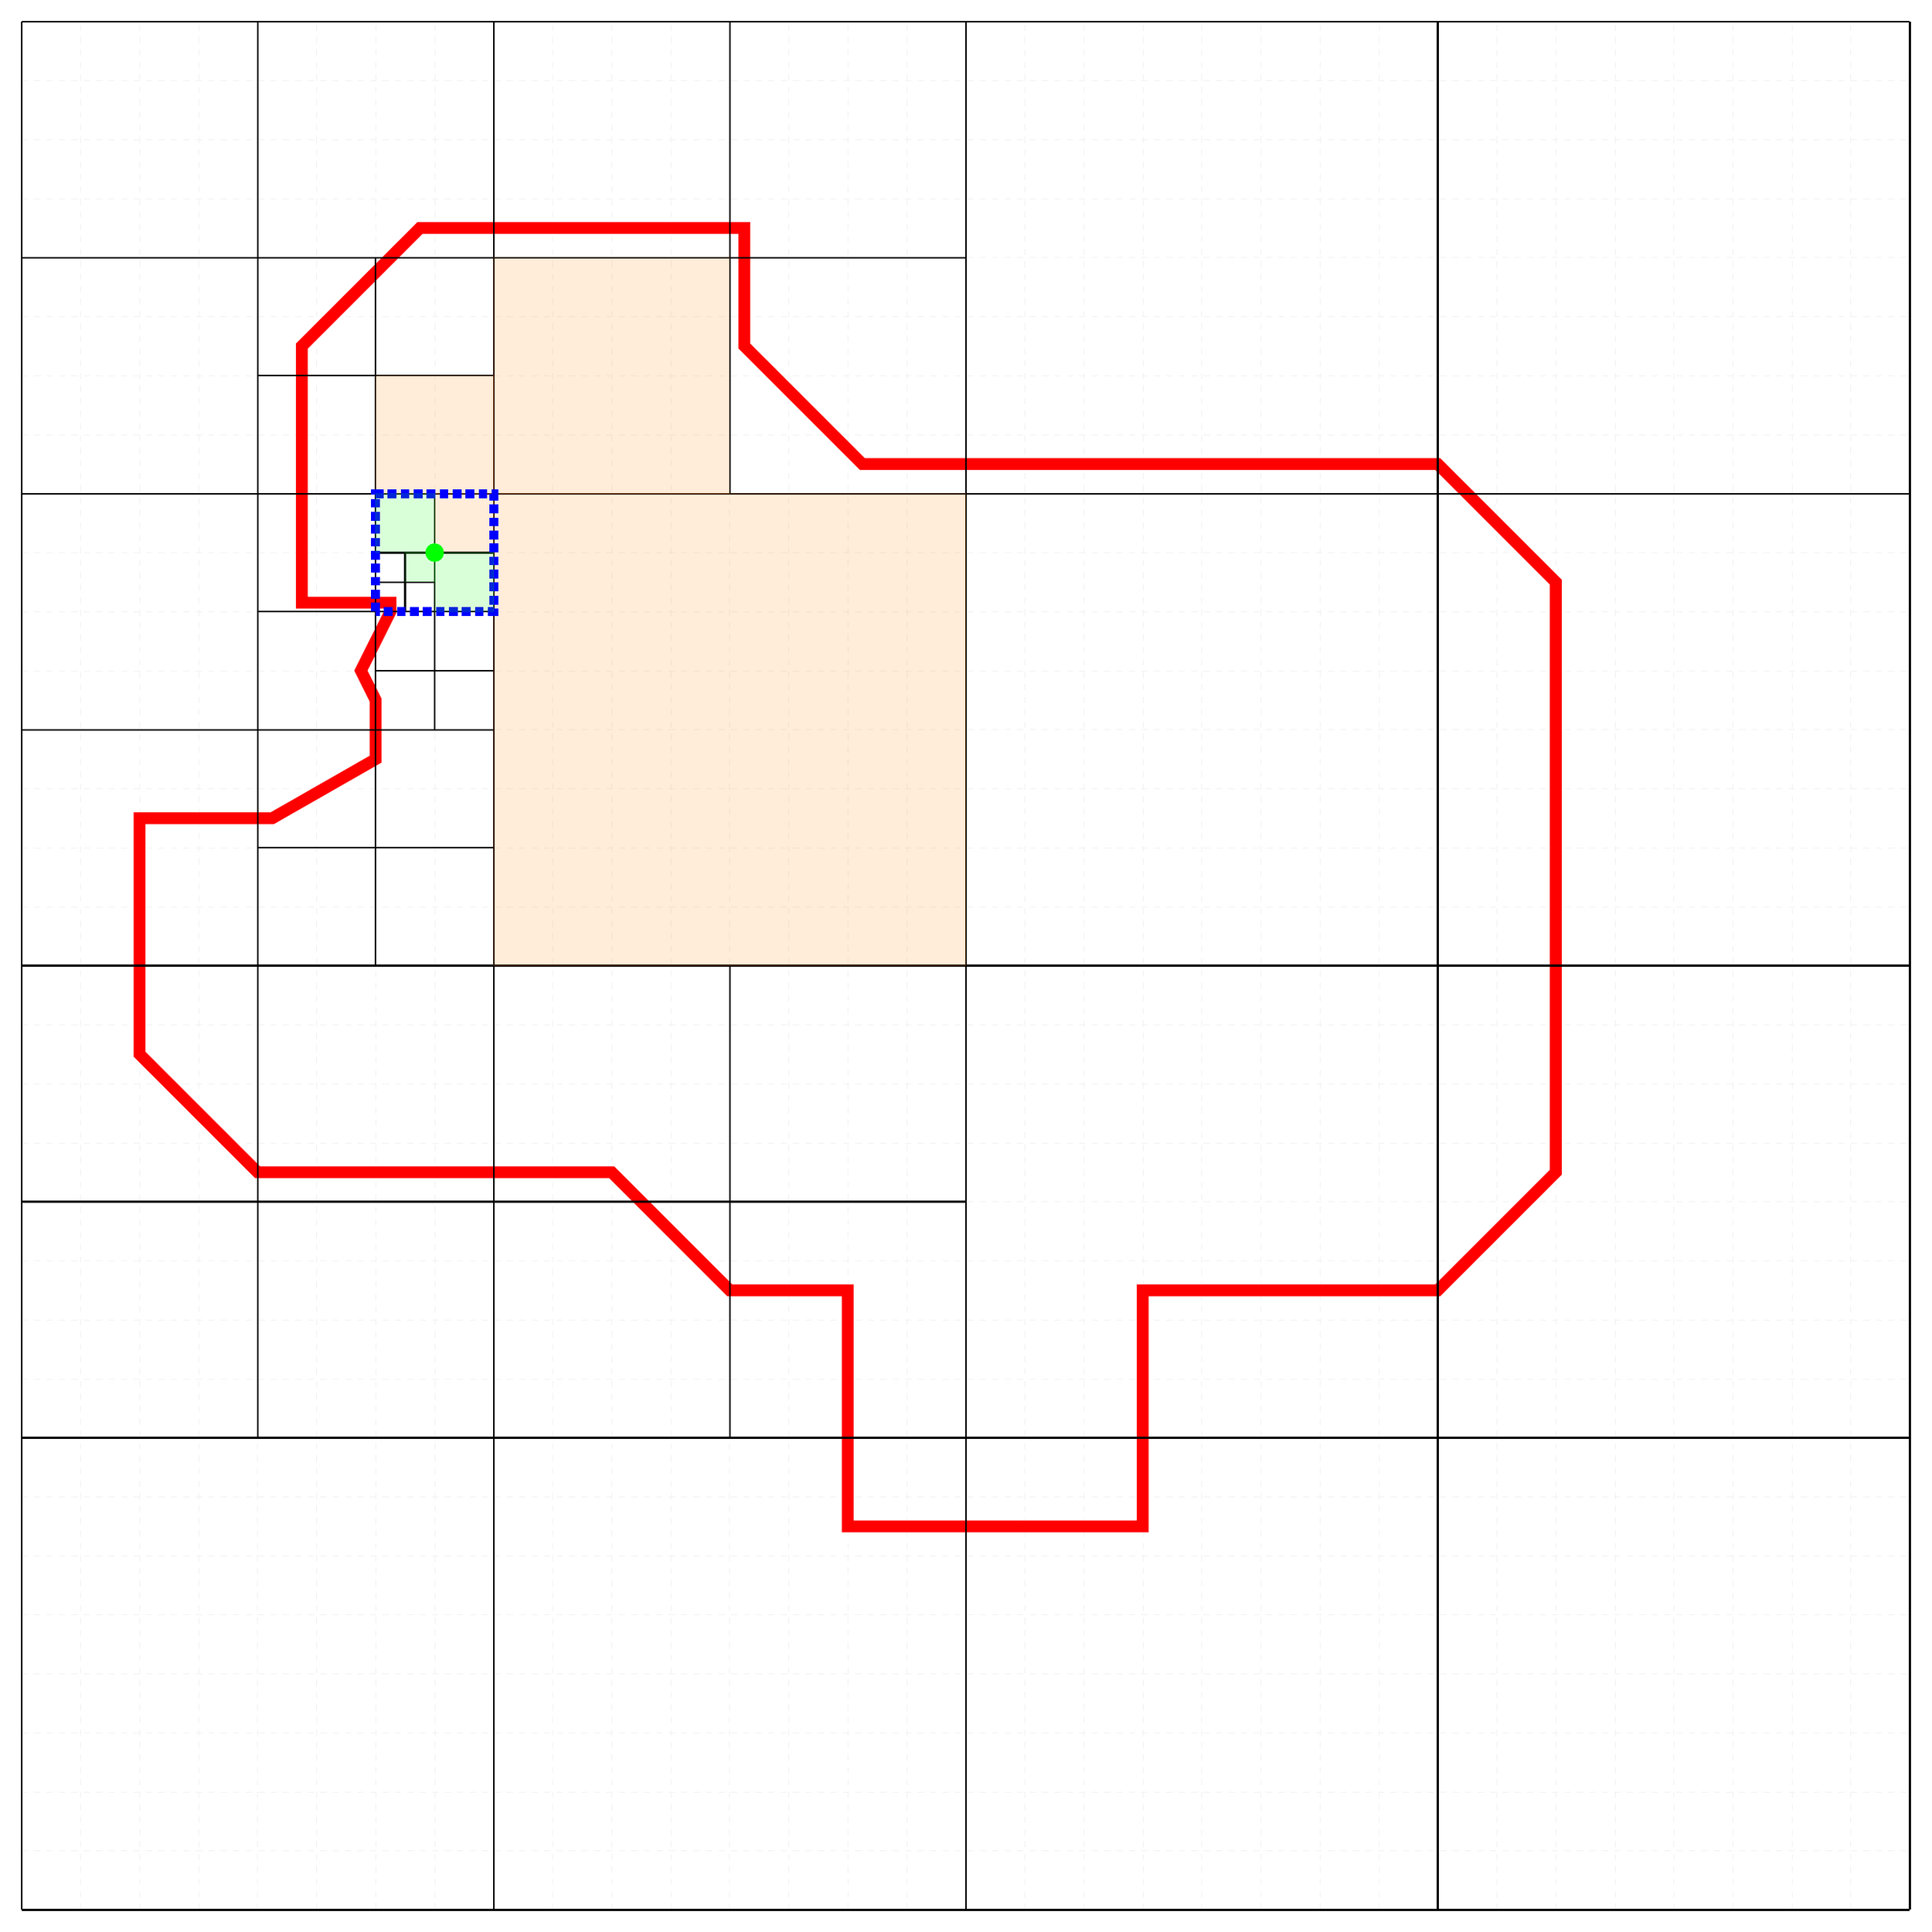
\begin{tikzpicture}
        \draw[step=1, very thin, light-gray, dashed] (0,0) grid (32,32);
        
        \node (start) at (6.25,22.25) {};
        \draw[poly] (start) -- ++(0,-0.25) -- ++(-0.25,-0.5) -- ++(-0.25,-0.5)  -- ++(0.25,-0.5)
            -- ++(0,-1) -- ++(-1.75,-1) -- ++(-2.25,0) -- ++(0,-4) -- ++(2,-2)
            -- ++(6,0) -- ++(2,-2) -- ++(2,0) -- ++(0,-4) -- ++(5,0) -- ++(0,4) -- ++(5,0) 
            -- ++(2,2) -- ++(0,10) -- ++(-2,2) -- ++(-9.75,0) -- ++(-2,2) 
            -- ++(0,2) -- ++(-5.5,0) -- ++(-2,-2) -- ++(0,-4.35) -- ++(1.6,0);
        \draw[step=8,  thick, black] (0,0)  grid (32,32);
        \draw[step=4,  thick, black] (0,24) grid (8,32);
        \draw[step=4,  thick, black] (0,16) grid (8,24);
        \draw[step=4,  thick, black] (0,8)  grid (8,16);
        \draw[step=4,  thick, black] (8,8)  grid (16,16);
        \draw[step=4,  thick, black] (8,24) grid (16,32);
        \draw[step=2,  thick, black] (4,16) grid (8,20);
        \draw[step=2,  thick, black] (4,20) grid (8,24);
        \draw[step=2,  thick, black] (4,24) grid (8,28);
        \draw[step=1,  thick, black] (6,20) grid (8,24);
        \draw[step=0.5,thick, black] (6,22) grid (7,23);

        \draw[orange, opacity=0.15, fill] (8,16) rectangle (16,24);
        \draw[orange, opacity=0.15, fill] (6,24) rectangle (8,26);
        \draw[orange, opacity=0.15, fill] (8,24) rectangle (12,28);
        \draw[orange, opacity=0.15, fill] (7,23) rectangle (8,24);
        
        \draw[blue, line width=1.5mm, dotted] (6,22) rectangle (8,24);
        
        \draw[green, opacity=0.15, fill] (6.5,22.5) rectangle (7,23);
        \draw[green, opacity=0.15, fill] (7,22) rectangle (8,23);
        \draw[green, opacity=0.15, fill] (6,23) rectangle (7,24);

        \draw[green, fill] (7,23) circle (0.15);
    \end{tikzpicture}
\end{page}

\begin{page}
    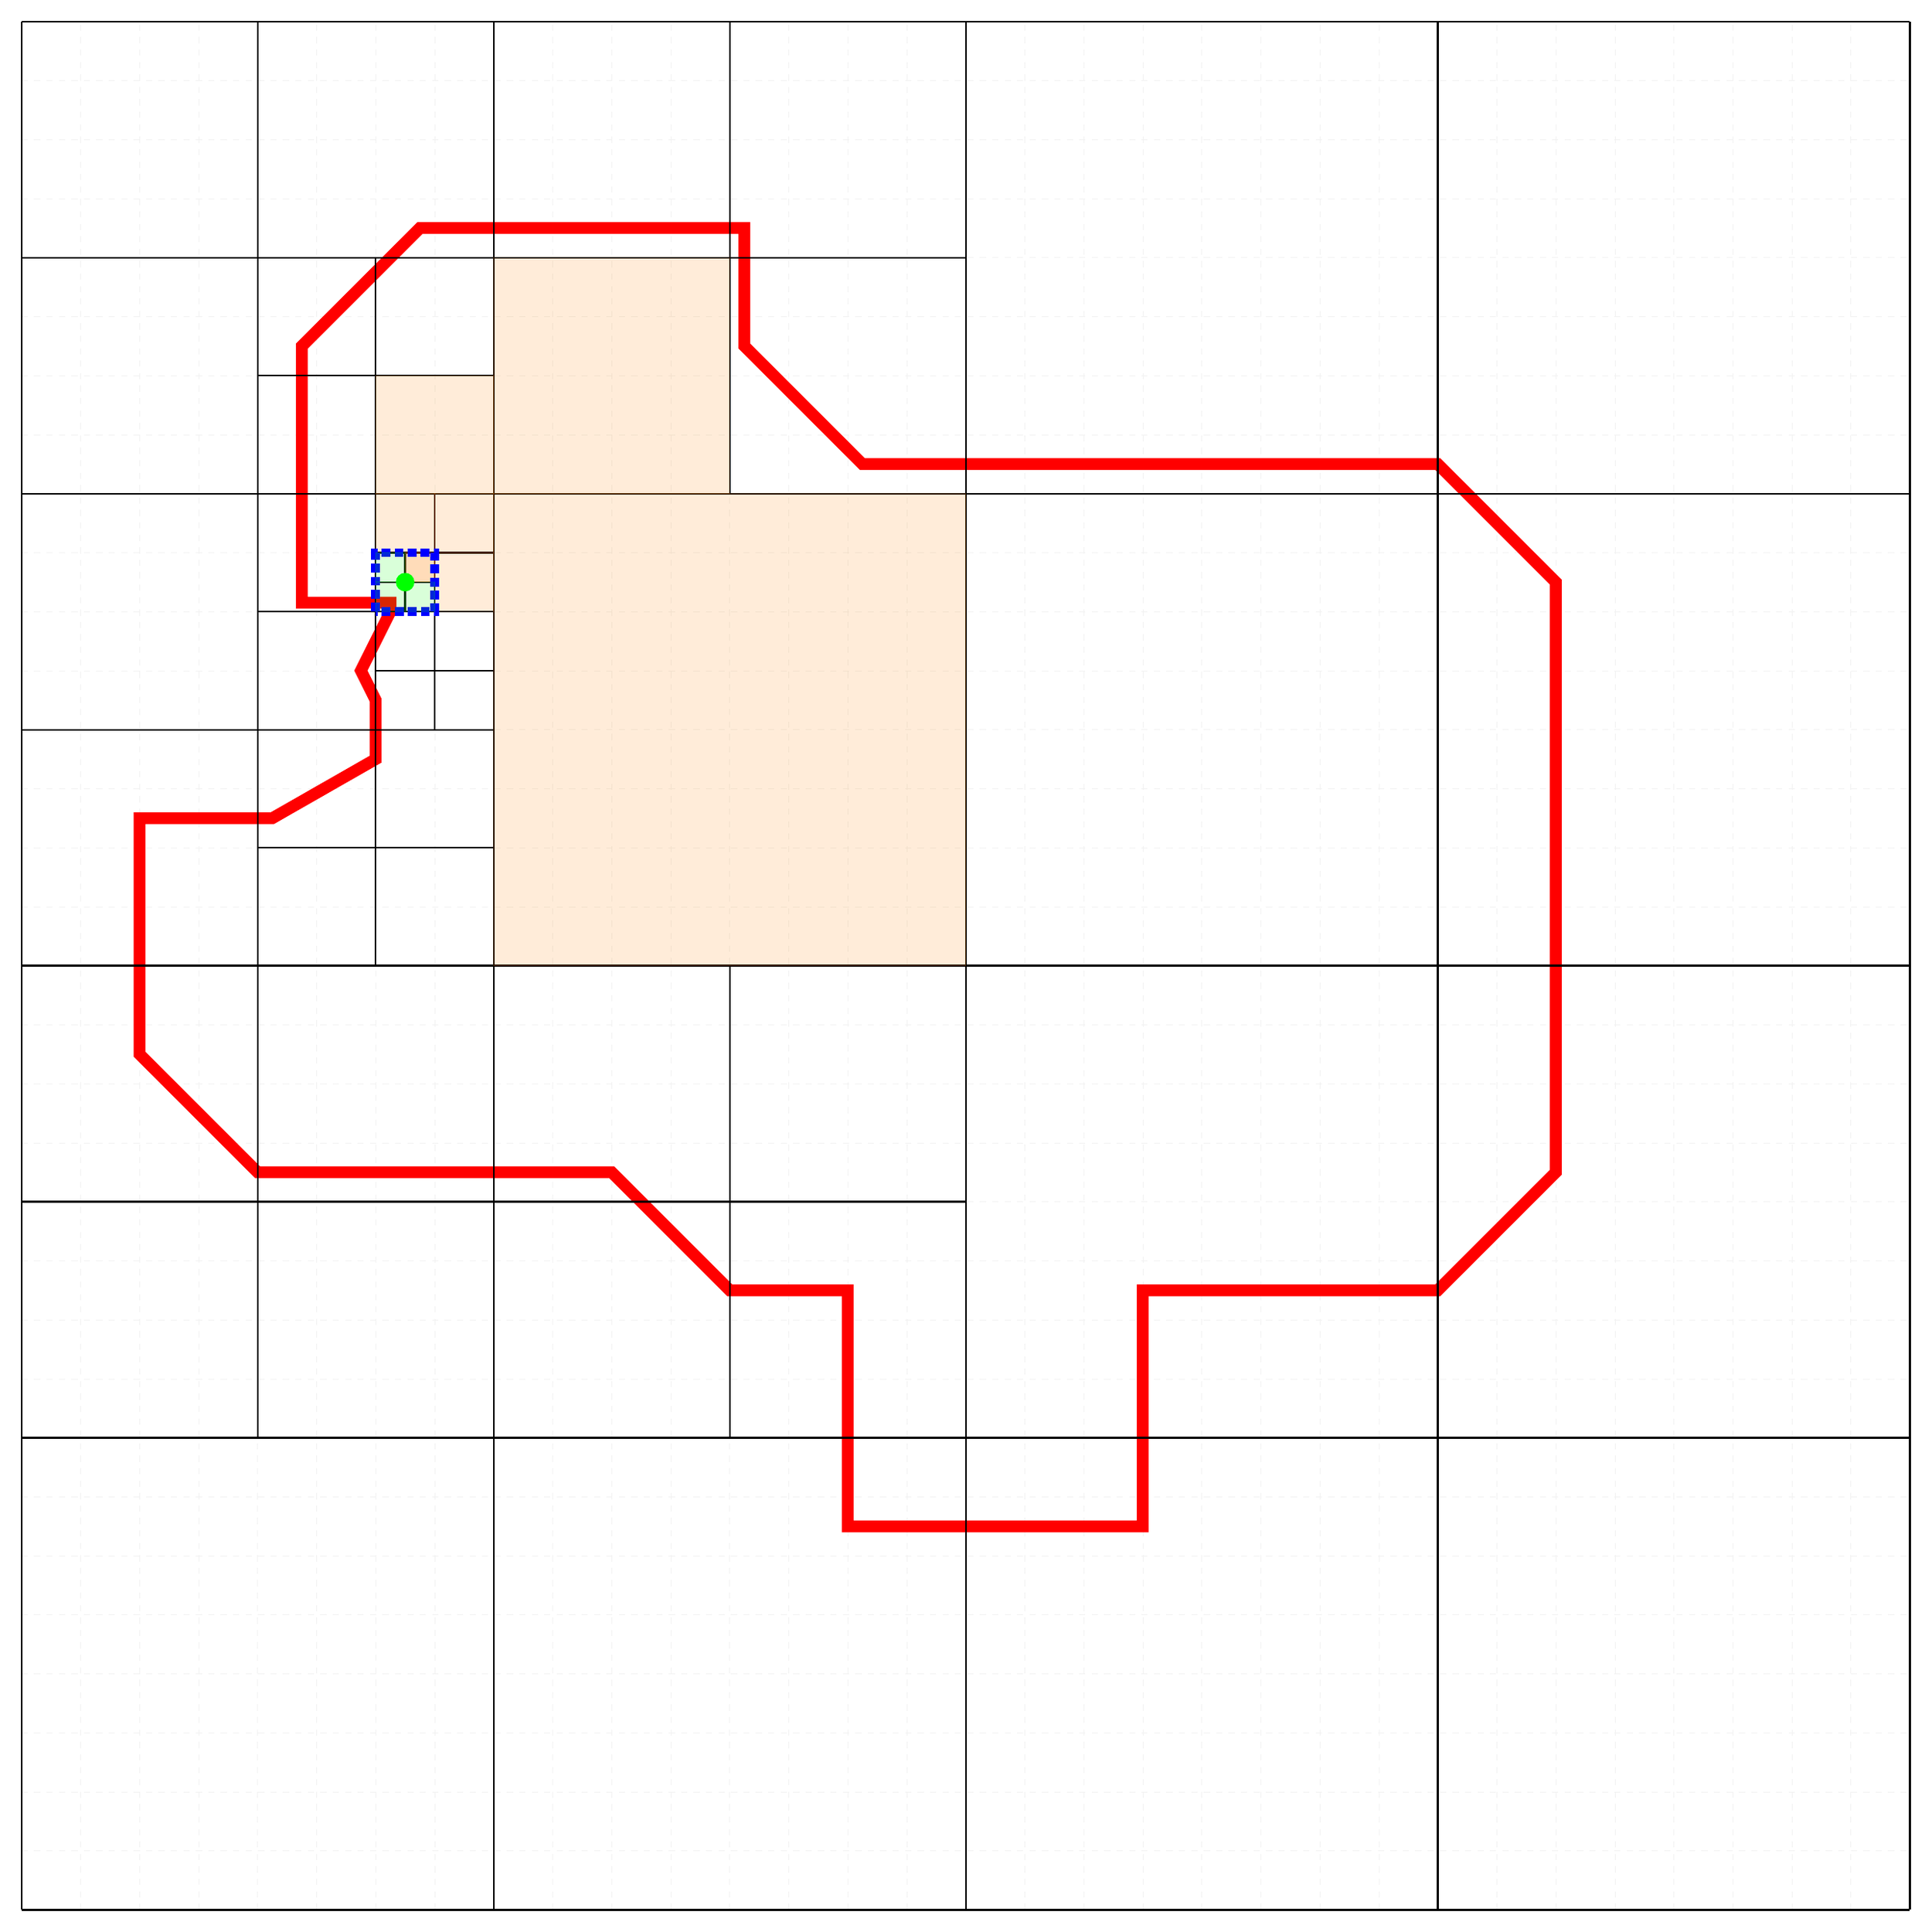
\begin{tikzpicture}
        \draw[step=1, very thin, light-gray, dashed] (0,0) grid (32,32);
        
        \node (start) at (6.25,22.25) {};
        \draw[poly] (start) -- ++(0,-0.25) -- ++(-0.25,-0.5) -- ++(-0.25,-0.5)  -- ++(0.25,-0.5)
            -- ++(0,-1) -- ++(-1.75,-1) -- ++(-2.25,0) -- ++(0,-4) -- ++(2,-2)
            -- ++(6,0) -- ++(2,-2) -- ++(2,0) -- ++(0,-4) -- ++(5,0) -- ++(0,4) -- ++(5,0) 
            -- ++(2,2) -- ++(0,10) -- ++(-2,2) -- ++(-9.75,0) -- ++(-2,2) 
            -- ++(0,2) -- ++(-5.5,0) -- ++(-2,-2) -- ++(0,-4.35) -- ++(1.6,0);
        \draw[step=8,  thick, black] (0,0)  grid (32,32);
        \draw[step=4,  thick, black] (0,24) grid (8,32);
        \draw[step=4,  thick, black] (0,16) grid (8,24);
        \draw[step=4,  thick, black] (0,8)  grid (8,16);
        \draw[step=4,  thick, black] (8,8)  grid (16,16);
        \draw[step=4,  thick, black] (8,24) grid (16,32);
        \draw[step=2,  thick, black] (4,16) grid (8,20);
        \draw[step=2,  thick, black] (4,20) grid (8,24);
        \draw[step=2,  thick, black] (4,24) grid (8,28);
        \draw[step=1,  thick, black] (6,20) grid (8,24);
        \draw[step=0.5,thick, black] (6,22) grid (7,23);

        \draw[orange, opacity=0.15, fill] (8,16) rectangle (16,24);
        \draw[orange, opacity=0.15, fill] (6,24) rectangle (8,26);
        \draw[orange, opacity=0.15, fill] (8,24) rectangle (12,28);
        \draw[orange, opacity=0.15, fill] (7,23) rectangle (8,24);
        \draw[orange, opacity=0.15, fill] (6.5,22.5) rectangle (7,23);
        \draw[orange, opacity=0.15, fill] (7,22) rectangle (8,23);
        \draw[orange, opacity=0.15, fill] (6,23) rectangle (7,24);
        \draw[orange, opacity=0.15, fill] (6.5,22.5) rectangle (7,23);
        
        \draw[blue, line width=1.5mm, dotted] (6,22) rectangle (7,23);
        
        \draw[green, opacity=0.15, fill] (6,22)   rectangle (6.5,22.5);
        \draw[green, opacity=0.15, fill] (6,22.5) rectangle (6.5,23);
        \draw[green, opacity=0.15, fill] (6.5,22) rectangle (7,22.5);

        \draw[green, fill] (6.5,22.5) circle (0.15);
    \end{tikzpicture}
\end{page}
\end{document} 
